\section{Jakub Kierznowski}
\label{sec:kierzno}
%\maketitle
%\begin{document}


%\documentclass{article}


\subsection{Ogólne informacje o psach}
Wszyscy wiemy, że
\[ \lim_{pieski \to\infty} pieski = słodkość ^\infty \]



Dzięki temu mamy piękne zdjęcie pieska \ref{fig:pies}


\begin{figure}[htbp]
    \centering
    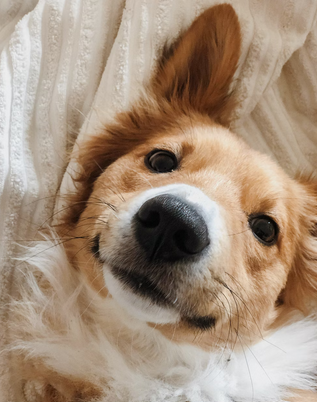
\includegraphics[scale=1, angle=90, width=\textwidth]{pictures/dog.png}
    \caption{Piesek czekający na głaskanie}
    \label{fig:pies}
\end{figure}


\subsection{Tabela}
Tabela \ref{tab:przedmioty} przedstawia ulubione przedmioty studentów ISI
\begin{table}[htbp]
\begin{tabular}{|l|c|c|r|}
\hline
\textbf{Nazwa}  & \textbf{Ilość wykładów}                                    & \textbf{Ilość ćwiczeń}                                     & \textbf{Czy enjoyable}                                               \\ \hline
    {\ul ALiGA}     & \cellcolor[HTML]{000000}{\color[HTML]{FFFFFF} \textit{28}} & \cellcolor[HTML]{000000}{\color[HTML]{FFFFFF} \textit{28}} & \cellcolor[HTML]{000000}{\color[HTML]{FFFFFF} \textit{Nie}}          \\ \hline
    {\ul Analiza}   & \cellcolor[HTML]{000000}{\color[HTML]{FFFFFF} \textit{42}} & \cellcolor[HTML]{000000}{\color[HTML]{FFFFFF} \textit{42}} & \cellcolor[HTML]{000000}{\color[HTML]{FFFFFF} \textit{Bardzo nie}}   \\ \hline
    {\ul Narzędzia} & \cellcolor[HTML]{000000}{\color[HTML]{FFFFFF} \textit{14}} & \cellcolor[HTML]{000000}{\color[HTML]{FFFFFF} \textit{14}} & \cellcolor[HTML]{000000}{\color[HTML]{FFFFFF} \textit{Jeszcze jak!}} \\ \hline
    {\ul Logika}    & \cellcolor[HTML]{000000}{\color[HTML]{FFFFFF} \textit{28}} & \cellcolor[HTML]{000000}{\color[HTML]{FFFFFF} \textit{14}} & \cellcolor[HTML]{000000}{\color[HTML]{FFFFFF} \textit{Przyjemne}}    \\ \hline
\end{tabular}
\label{tab:przedmioty}
\end{table}



\subsection{Matematyczne wzorki z dzisiejszej algebry}
\begin{enumerate}
    \item takie macierze liczymy:
        $$\begin{bmatrix}
            5&0&-3&1\\
            5&2&-2&0\\
            -5&1&4&2\\
            0&7&6&1
        \end{bmatrix}$$
    \item można to zapisać też jako:
        $$\begin{cases}
            5x - 3z = 1\\
            5x + 2y - 2z = 0\\
            -5x + y - 4z = 2\\
            7y + 6z = 1
        \end{cases}$$
    \item inne dziwne wzory, które miejmy nadzieję \textbf{nikt} nie sprawdzi
    $$\begin{case}
         \[ \int_{-\infty}^{\infty} \Delta
    = \,dx \sum_{(\mathbf{x},\mathbf{s})\in \mathcal R}
       \log \sin{ (\mathbf{s}\mid\mathbf{x})} - \sum_{i=1}^\infty
       \frac{\Psi}{\pi^2} \]
        \end{case}$$
    \end{enumerate}

\subsection{Listy i inne ekwipunki}

    \begin{itemize}
        \item pierwsze \verb|itemize|
        \item drugie
        \item trzecie
    \end{itemize}

    \begin{enumerate}
        \item Pierwsze \verb|enumerate|
        \item Drugie
        \item Trzecie
    \end{enumerate}



\newpage
\subsection{Memy z Francuzami}
\textit {(to nie jest atak na nich, uwielbiam bagietki i inne rogale)}
    \begin{figure}[htbp]
    \centering
    \begin{minipage}[b]{0.4\textwidth}
        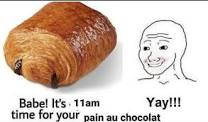
\includegraphics[width=\textwidth]{pictures/chocolat.jpg}
        \caption{Francuzi o 11}
        \label{fig:pain}
    \end{minipage}
    \begin{minipage}[b]{0.4\textwidth}
        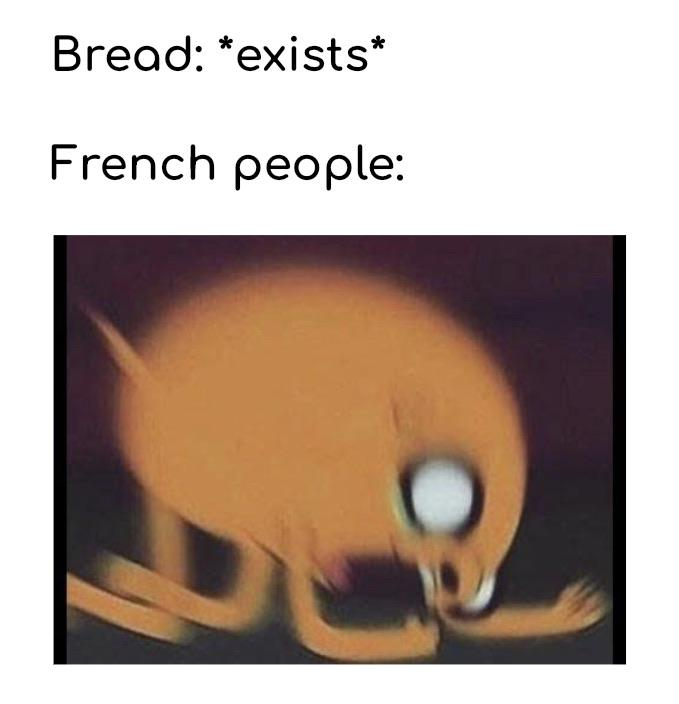
\includegraphics[width=\textwidth]{pictures/french.jpg}
        \caption{Ból chleba}
        \label{fig:pain2}
    \end{minipage}
    \end{figure}

\subsection{Krótki tekst od GPT 3.5}
    \begin{group}
    
    Magic \textbf{Delphin} and his fiery friend, aptly named Fire, embarked on an extraordinary adventure in the heart of the majestic Alps. \textbf{Delphin}, a wizard of \textit{considerable skill}, possessed a \textit{deep connection} with the natural world \ref{fig:pies}, while Fire was a mischievous elemental spirit who could manipulate flames at will. Together, they set out to explore the breathtaking landscapes, their journey beginning in a small village nestled among the towering peaks.
    
\vspace{.5cm}

    Their adventure took them through enchanted forests where trees whispered secrets and animals greeted them with curious eyes. \textbf{Delphin's} magical abilities allowed him to converse with the flora and fauna, creating a harmonious bond with the ALPINE ecosystem. Fire, on the other hand, brought warmth to the cold mountain nights and illuminated their path with brilliant displays of fire dances. Along their way, they discovered \textbf{hidden} caves filled with ancient artifacts, crossed crystal-clear streams, and scaled treacherous cliffs. In the heart of the Alps, they encountered a mysterious sorceress who revealed the \textbf{hidden} secrets of the mountains and granted them the wisdom to protect these sacred lands. Magic \textbf{Delphin} and Fire returned to their village as heroes, their souls forever intertwined with the magic of the ALPS, promising to safeguard this wondrous place for generations to come.
    
    \end{group}



%\end{document}